\chapter{Object Detection using SSD Mobilenet V2}

In this project, I developed a object detection model based on the SSD Mobilenet V2 version with the purpose of detecting four different objects (cola fanta sprite water). The focus was detecting and counting objects in minibar with best accuracy. During the project, different datasets trained for getting best results. The process and results are discussed below. 

\section{Training steps}

The model is trained in 40000 steps and 16 batch size.
\begin{figure}[!htbp]
    \centering
    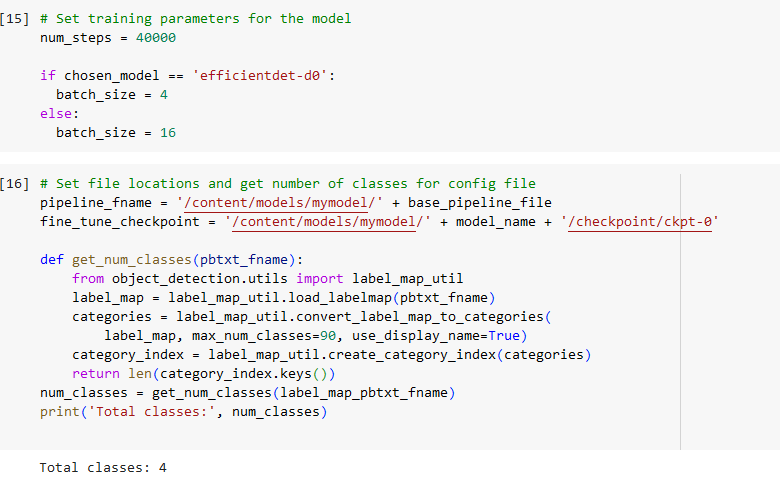
\includegraphics[width=1\textwidth]{Imgs/parameters.PNG}
    \caption{\label{fig:parameters}Parameters }
\end{figure}

\begin{figure}[!htbp]
    \centering
    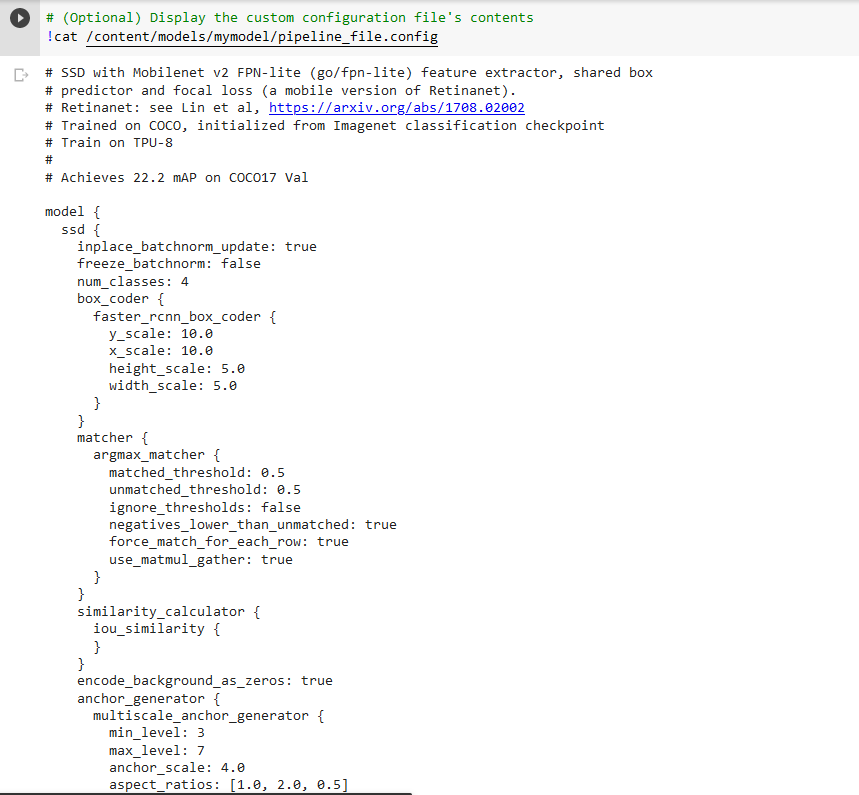
\includegraphics[width=0.6\textwidth]{Imgs/trainconfig.png}
    \caption{\label{fig:train_config}Parameters }
\end{figure}
\begin{figure}[!htbp]
    \centering
    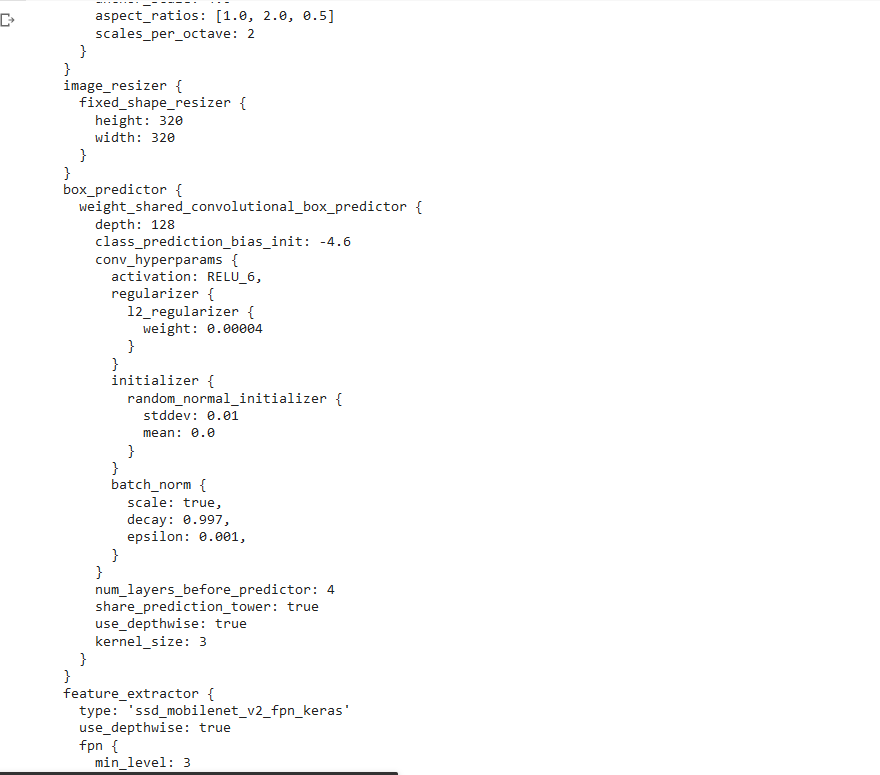
\includegraphics[width=0.6\textwidth]{Imgs/trainconfig2.png}
    \caption{\label{fig:train_config}Parameters }
\end{figure}
\begin{figure}[!htbp]
    \centering
    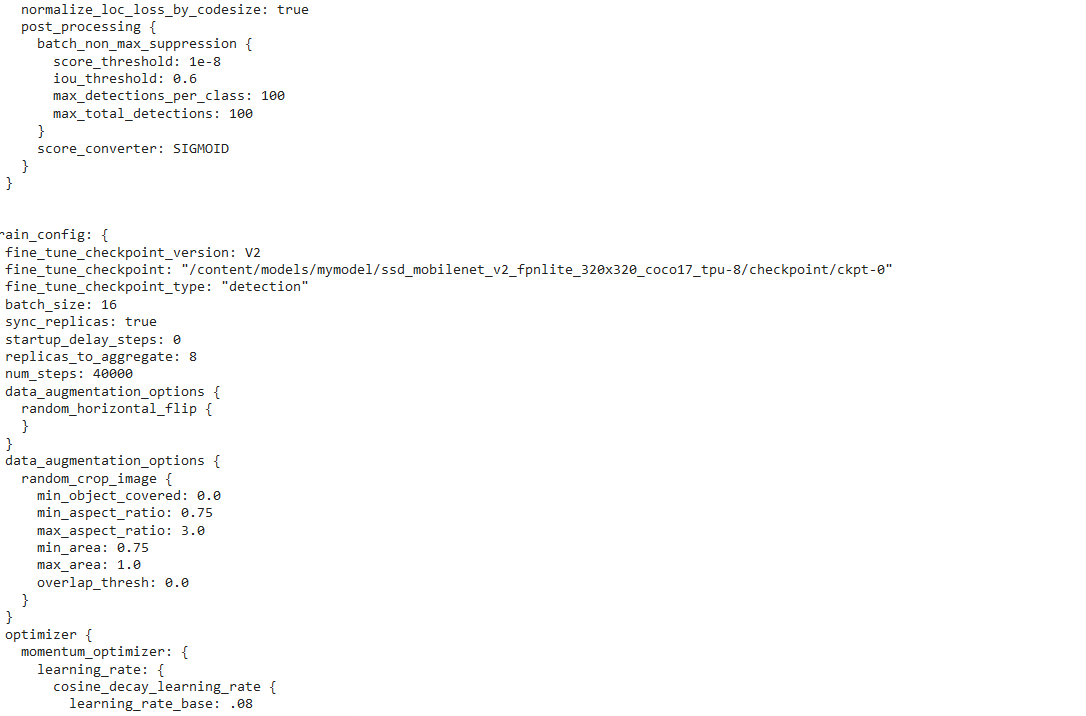
\includegraphics[width=0.6\textwidth]{Imgs/training_parameters.png}
    \caption{\label{fig:train_params}Parameters }
\end{figure}

\subsection{Training Results}
Threshold results of training:
\begin{figure}[!htbp]
    \centering
    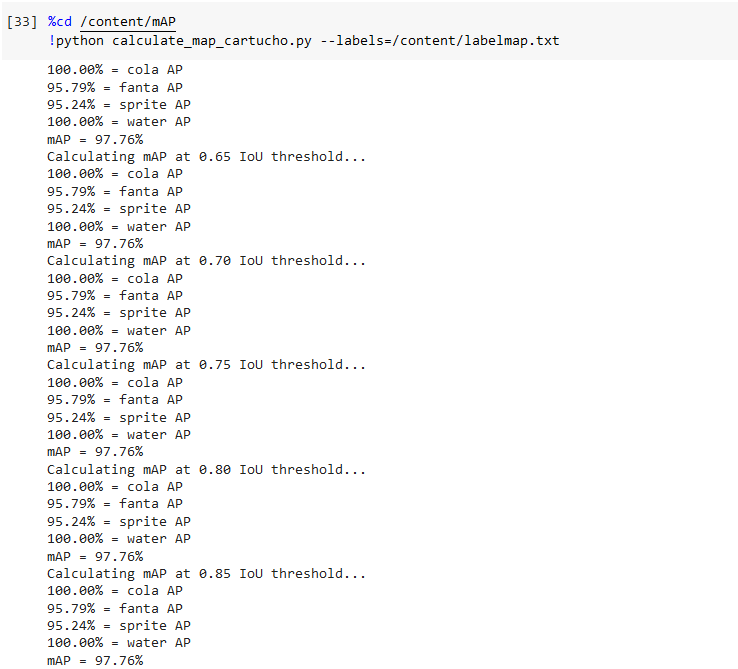
\includegraphics[width=0.6\textwidth]{Imgs/threshold1.PNG}
    \caption{\label{fig:threshold}Threshold }
\end{figure}
\begin{figure}[!htbp]
    \centering
    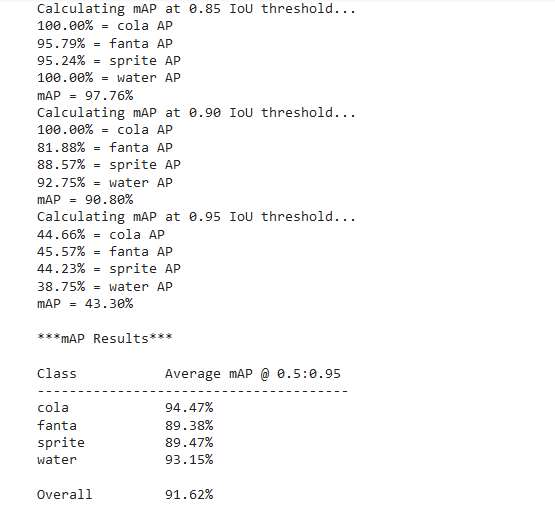
\includegraphics[width=0.6\textwidth]{Imgs/threshold2.PNG}
    \caption{\label{fig:threshold}Threshold }
\end{figure}

\subsection{Learning rate and loss of model}
Here is the rate of model learning. We can see that learning rate schedules in deep learning models often involve an initial phase where the learning rate is relatively high, followed by a gradual decrease over time. This pattern of a learning rate that "peaks" before decreasing serves several purposes.

\begin{figure}[!htbp]
    \centering
    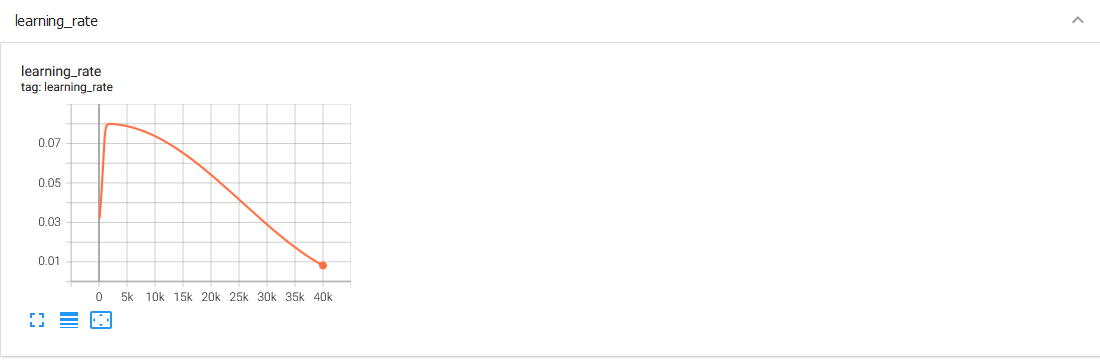
\includegraphics[width=0.8\textwidth]{Imgs/learning_rate.png}
    \caption{\label{fig:learning_rate}Learning rate}
\end{figure}
\\

Loss is s a measure of how well a model's predictions align with the true values or labels of the training data. The loss quantifies the error or mismatch between the predicted output of the model and the desired output.

During the training process, the model iteratively adjusts its parameters or weights to minimize the loss. By minimizing the loss, the model aims to improve its ability to make accurate predictions on unseen data.

\begin{figure}[!htbp]
    \centering
    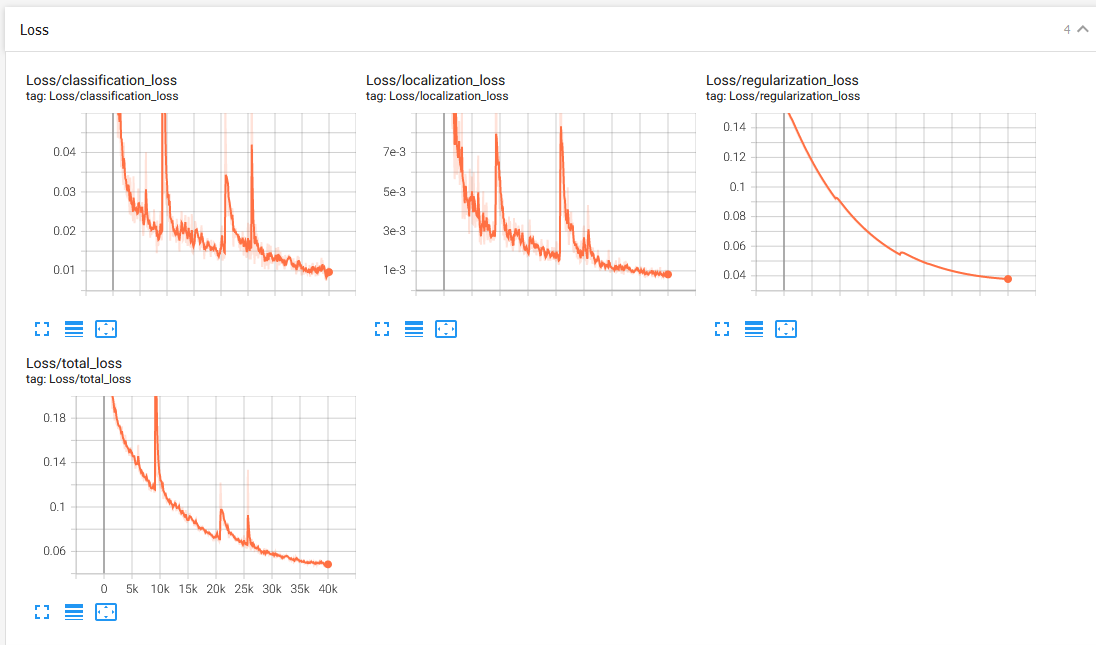
\includegraphics[width=0.9\textwidth]{Imgs/loss.PNG}
    \caption{\label{fig:loss}Loss}
\end{figure}

Detecting and counting four object:

\begin{figure}[!htbp]
    \centering
    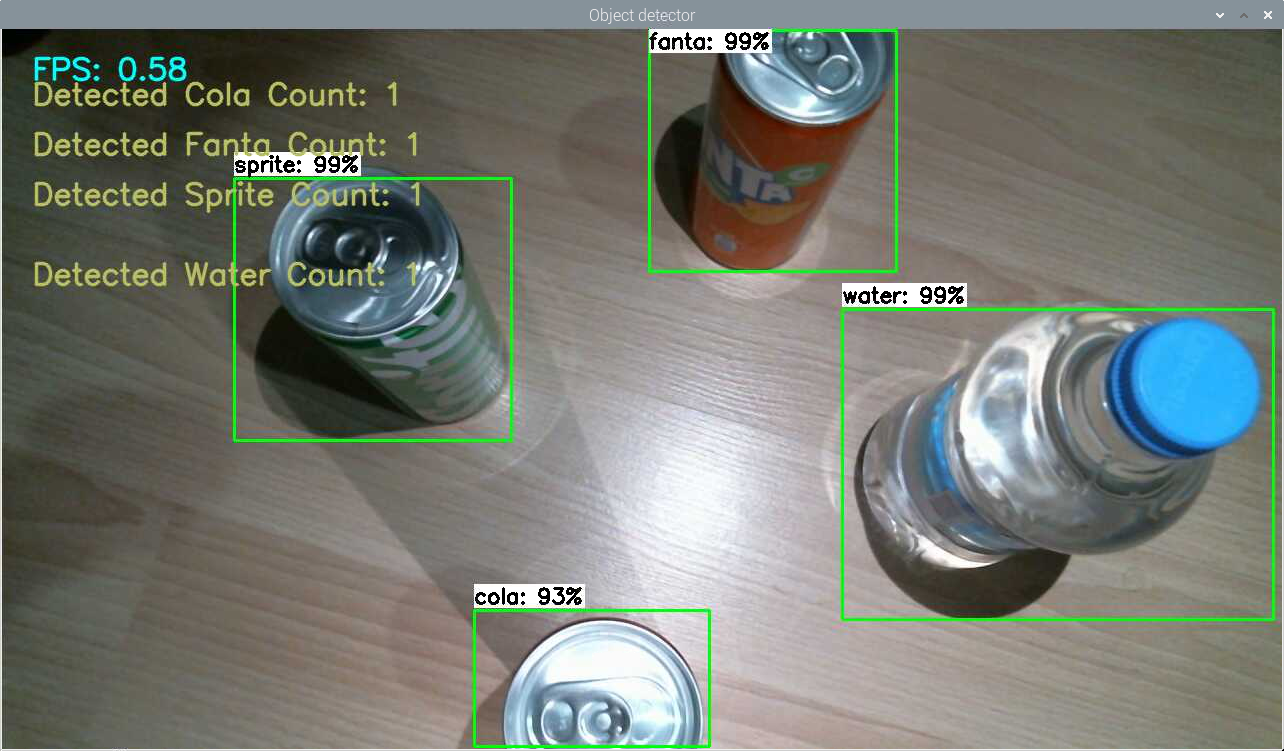
\includegraphics[width=0.9\textwidth]{Imgs/object_counts.PNG}
    \caption{\label{fig:loss}Object Detection and Counts}
\end{figure}

